\chapter{MixVRTの実装}\label{cha:Implementation}
本章では、\toolName の実装について説明する。
\toolName のシステム構成(仮)を、図\ref{fig:System}に示す。
\begin{figure}[tp]
    \begin{center}
        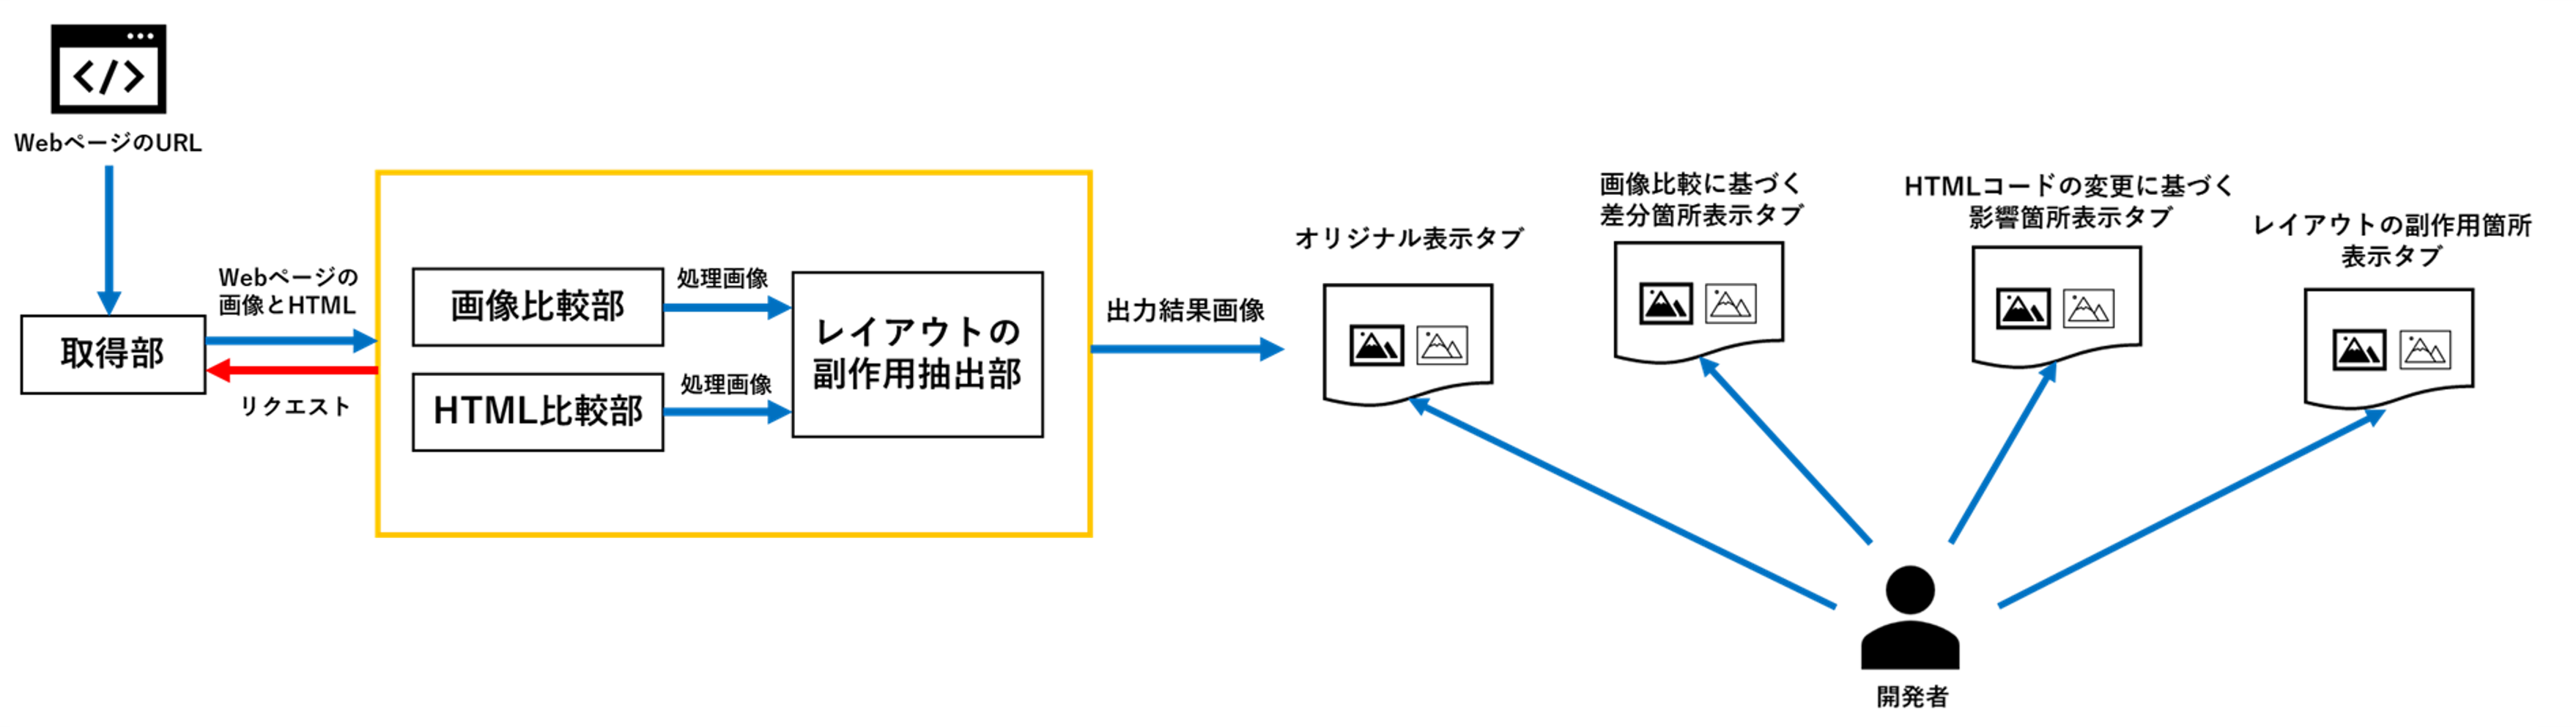
\includegraphics[width=1.0\columnwidth]{image/4_System.png}
        \caption{\toolName のシステム構成(仮)}
        \label{fig:System}
    \end{center}
\end{figure}
% 私の開発したツールは、まずユーザーがWebページのURLを入力します。
% このURLを受け取ると、ツールは該当するWebページから画像を取得し、
% これらの画像に対して特定の処理を行います。処理された画像は"static/images"ディレクトリに保存されます。
% そして、Flaskがローカルサーバを提供し、
% "templates"フォルダにあるHTMLコードが"static/images"ディレクトリを参照できるようになっています。
% この仕組みにより、ユーザーはローカルに立てられたFlaskサーバを通じて、
% Webページ上で生成された画像を確認することができます。
本研究では、\toolName の試作にあたり、以下の5つの処理部を実装する。
\begin{itemize}
    \item 取得部
    \item 画像比較部
    \item HTML比較部
    \item レイアウトの副作用抽出部
    \item レイアウトの不具合抽出部
          % \item インターフェース表示部
\end{itemize}
% \begin{itemize}
%     \item 取得部
%     \item 画像比較部
%           \begin{enumerate}
%               \item 差分箇所検出
%           \end{enumerate}
%     \item HTML比較部
%           \begin{enumerate}
%               \item 差分コード生成
%               \item 差分コード解析
%               \item 影響箇所強調HTMLコード生成
%           \end{enumerate}
%     \item レイアウトの副作用箇所抽出部
%     \item インターフェース表示部
% \end{itemize}
以降、\toolName を構成する5つの処理部について説明する。
\par

\section{取得部}\label{sec:Web_data_get_section}
取得部は、WebページのURLを入力として受け取り、Webページの画像とHTMLコードを取得する。
取得したWebページの画像は画像比較部(\ref{sec:Difference_extraction_section}節で後述)に出力し、取得したWebページのHTMLコードはHTML比較部(\ref{sec:Affected_area_extraction}節で後述)に出力する。
なお、HTML比較部が取得部にWebページのURLを与えて呼び出す場合においては、Webページの画像のみをHTML比較部に出力する。
Webページの画像取得には、Selenium WebDriver(\ref{sec:Selenium_WebDriver}節を参照)を用いてWebページの画像を取得する。
Selenium WebDriverを用いて取得したWebページの画像例を、図\ref{fig:4_get_images}に示す。
\begin{figure}[tp]
    \begin{center}
        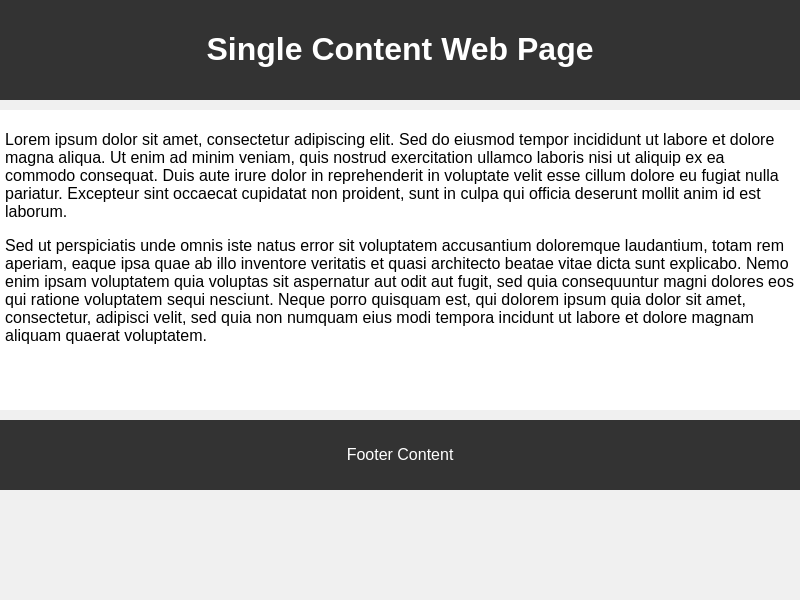
\includegraphics[width=1.0\columnwidth]{image/4_get_images.png}
        \caption{Selenium WebDriverを用いて取得したWebページの画像例}
        \label{fig:4_get_images}
    \end{center}
\end{figure}
WebページのHTMLコード取得には、Pythonライブラリの一つであるrequestsモジュール(\ref{sec:requests}節を参照)を用いて、WebページのURLからWebページのHTMLコードを取得する。
requestsモジュールを用いて取得したWebページのHTMLコード例を、ソースコード\ref{lst:html_example}に示す。
\begin{lstlisting}[language=HTML, caption=requestsモジュールを用いて取得したWebページのHTMLコード例, label=lst:html_example]
    <!DOCTYPE html>
    <html lang="en">
    
    <head>
        <meta charset="UTF-8">
        <meta name="viewport" content="width=device-width, initial-scale=1.0">
        <title>Single Content Web Page</title>
        <style>
            body {
                font-family: Arial, sans-serif;
                margin: 0;
                padding: 0;
                background-color: #f0f0f0;
            }
    
            header {
                background-color: #333;
                color: white;
                text-align: center;
                padding: 10px 0;
            }
    
            .container {
                height: 300px auto;
                width: 100%;
                margin: 10px auto;
                overflow: hidden;
            }
    
            .main-content {
                height: 300px;
                background-color: #fff;
                padding: 5px;
                box-sizing: border-box;
            }
    
            footer {
                background-color: #333;
                color: white;
                text-align: center;
                padding: 10px 0;
                clear: both;
            }
        </style>
    </head>
    
    <body>
        <header>
            <h1>Single Content Web Page</h1>
        </header>
        <div class="container">
            <div class="main-content">
                <p>Lorem ipsum dolor sit amet, consectetur adipiscing elit. Sed do eiusmod tempor incididunt ut labore et
                    dolore magna aliqua. Ut enim ad minim veniam, quis nostrud exercitation ullamco laboris nisi ut aliquip
                    ex ea commodo consequat. Duis aute irure dolor in reprehenderit in voluptate velit esse cillum dolore eu
                    fugiat nulla pariatur. Excepteur sint occaecat cupidatat non proident, sunt in culpa qui officia
                    deserunt mollit anim id est laborum.</p>
                <p>Sed ut perspiciatis unde omnis iste natus error sit voluptatem accusantium doloremque laudantium, totam
                    rem aperiam, eaque ipsa quae ab illo inventore veritatis et quasi architecto beatae vitae dicta sunt
                    explicabo. Nemo enim ipsam voluptatem quia voluptas sit aspernatur aut odit aut fugit, sed quia
                    consequuntur magni dolores eos qui ratione voluptatem sequi nesciunt. Neque porro quisquam est, qui
                    dolorem ipsum quia dolor sit amet, consectetur, adipisci velit, sed quia non numquam eius modi tempora
                    incidunt ut labore et dolore magnam aliquam quaerat voluptatem.</p>
            </div>
        </div>
        <footer>
            <p>Footer Content</p>
        </footer>
    </body>
    
    </html>
\end{lstlisting}

\section{画像比較部}\label{sec:Difference_extraction_section}
画像比較部は、取得部からWebページの変更前画像と変更後画像を受け取り、画像比較に基づく差分箇所を色付きの枠で囲んで強調表示したWebページの変更前画像と変更後画像を生成する。
また、それらの画像から枠のみを残してそれ以外の部分を黒くすることで、差分箇所を囲む色付きの枠のみを抽出した、変更前画像と変更後画像も生成する。
なお、差分箇所を囲む色付きの枠のみを抽出した、変更前画像と変更後画像に関しては、レイアウトの副作用抽出部に処理画像として出力する。
画像比較部の処理の流れを、以下に示す。
\begin{enumerate}
    \item 高解像度画像生成処理
    \item 適応的二値化処理
    \item 差分検出処理
    \item 膨張処理
    \item 輪郭検出処理
    \item 枠描画処理
\end{enumerate}
以降、画像比較部の各処理について説明する。

\subsection{高解像度画像生成処理}\label{subsec:Generate_high_images}
高解像度画像生成処理は、Webページの画像から高解像度画像を生成する。高解像度画像は、輪郭検出処理(\ref{subsec:contour_detection_processing}節で後述)の精度を向上するために必要である。
高解像度画像を生成する流れを、以下に示す。なお、リサイズに使用するアルゴリズムには、LANCZOSフィルタ(\ref{sec:pillow}を参照)を用いる。
\begin{enumerate}
    \item PillowのImage.open関数(\ref{sec:pillow}節を参照)を用いて、Webページの画像をImageオブジェクトとして読み込む。
    \item 画像の拡大率を設定する。本研究では、$2$とする。
    \item Imageオブジェクトから画像の幅と高さを取得する。
    \item 画像の幅と高さにそれぞれ画像の拡大率を掛けた画像にリサイズする。
    \item リサイズした高解像度画像を保存する。
\end{enumerate}

\subsection{適応的二値化処理}\label{subsec:Adaptive_Binarisation}
適応的二値化処理は、Webページの画像の二値化(白黒化)を行う。
Webページの画像を二値化する流れを、以下に示す。
\begin{enumerate}
    \item OpenCVのimread関数(\ref{sec:opencv}を参照)を用いて、Webページの画像パスから画像を読み込む。
    \item OpenCVのcvtColor関数(\ref{sec:opencv}を参照)を用いて、画像をグレースケール化する。
    \item OpenCVのadaptiveThreshold関数(\ref{sec:opencv}を参照)を用いて、画像の二値化を行う。
\end{enumerate}

\subsection{差分検出処理}\label{subsec:difference_detection_process}
差分検出処理は、OpenCVのsubtract関数(\ref{sec:opencv}節を参照)を用いて、Webページの変更前画像と変更後画像の画像間で差分検出を行う。
差分検出処理により、Webページの変更前画像で削除された箇所とWebページの変更後画像で追加された箇所である差分箇所を検出できる。

\subsection{膨張処理}\label{subsec:dilation}
差分検出処理の後に膨張処理(\ref{sec:dilation}節を参照)を適用することで、
差分箇所の輪郭検出処理(\ref{subsec:contour_detection_processing}節で後述)を高める。
差分検出で生成した画像に対して、膨張処理を適用する流れを、以下に示す。
\begin{enumerate}
    \item 特定の形状とサイズを持つカーネルを設定する。本研究では、5x5ピクセルの正方形カーネルを採用する。
    \item 設定したカーネルを用いて、差分検出画像に膨張処理を適用する。適用後、画像内の差分箇所が拡大し、隣接する差分箇所が連結する。
    \item 膨張処理を複数回実行する。本研究では、膨張処理を6回繰り返すことで差分箇所を強調する。
\end{enumerate}

\subsection{輪郭検出処理}\label{subsec:contour_detection_processing}
輪郭検出処理は、OpenCVのfindContours関数(\ref{sec:opencv}節を参照)を用いて、膨張処理を適用した差分箇所を枠で囲む輪郭を検出する。
輪郭検出処理により、Webページの画像上における画面要素単位の差分箇所の輪郭座標を取得できる。

\subsection{枠描画処理}\label{subsec:Bounding box drawing process}
枠描画処理は、Webページの変更前画像と変更後画像に対して、
輪郭検出処理(\ref{subsec:Bounding box drawing process}節を参照)で取得した輪郭座標を用いて、
Webページの変更前画像で削除された箇所を赤枠で囲んだ画像と、Webページの変更後画像で追加された箇所を緑枠で囲んだ画像を生成する。
また、Webページの変更前画像と変更後画像のそれぞれと同じサイズの黒画像に対しても、
輪郭検出処理で取得した輪郭座標を用いて、
差分箇所を囲む色付きの枠のみを抽出した、変更前画像と変更後画像を生成する。
枠描画処理の流れを、以下に示す。
\begin{enumerate}
    \item cv2.boundingRect関数(\ref{sec:opencv}節を参照)を用いて、輪郭を取り囲む矩形の座標と幅、高さを取得する。
    \item 取得した矩形情報を引数に指定したcv2.rectangle関数(\ref{sec:opencv}節を参照)を用いて、画像上に色付きの枠を描画する。
\end{enumerate}


\section{HTML比較部}\label{sec:Affected_area_extraction}
HTML比較部は、取得部からWebページの変更前HTMLコードと変更後HTMLコードを受け取り、
HTMLコードの変更に基づく影響箇所を色付きの枠で囲んで強調表示した、Webページの変更前画像と変更後画像を生成する。
また、それらの画像から枠のみを残してそれ以外の部分を黒くすることで、影響箇所を囲む色付きの枠のみを抽出した、変更前画像と変更後画像も生成する。
なお、影響箇所を囲む色付きの枠のみを抽出した、変更前画像と変更後画像に関しては、レイアウトの副作用抽出部に処理画像として出力する。
HTML比較部の処理の流れを、以下に示す。
\begin{enumerate}
    \item 差分コード生成処理
    \item 差分コード解析処理
    \item 影響箇所強調HTMLコード生成処理
    \item 枠抽出処理
\end{enumerate}
以降、HTML比較部の各処理について説明する。

\subsection{差分コード生成処理}\label{subsec:diff_file_generate}
差分コード生成処理は、Webページの変更前HTMLコードと変更後HTMLコードを行ごとに比較して、差分コードをtxt形式として生成する。
なお、生成した差分コードは、コードの追加行には"+", 削除行には"-", 変更前後のHTMLコードにどちらにも存在しない行には"?"が先頭に付き、"?"を除いた差分コードを解析対象とする。
差分コードを生成する処理を、以下に示す。
\begin{enumerate}
    \item 変更前HTMLコードと変更後HTMLコードをそれぞれHTMLデータとして読み込む。
    \item difflibモジュール(\ref{sec:difflib}節を参照)を使用して、2つのHTMLデータ間を行ごとに比較する。
    \item 差分コードをtxt形式で保存する
\end{enumerate}



\subsection{差分コード解析処理}\label{subsec:diff_file_analyze}
差分コード解析処理は、差分コード生成処理から差分コードを受け取り、差分コードからbody要素内の変更箇所とstyle要素内の変更箇所を見つける。

\subsection{枠付けHTMLコード生成処理}\label{subsec:modified_html_generate}
枠付けHTMLコード生成処理は、差分コード解析処理から変更箇所を受け取り、変更箇所に色付きの枠をつけるcssクラスを追加したHTMLコードを生成する。
なお、変更箇所に色付きの枠をつけるcssクラスを追加したHTMLコードを、枠付けHTMLコードと定義する。

\subsection{枠抽出処理}\label{subsec:frame_extraction}
枠抽出処理は、Webページの変更前画像と枠付けを行ったWebページの変更前画像を比較し、赤枠のみを抽出した画像を生成する。
また、Webページの変更後画像と枠付けを行ったWebページの変更後画像を比較し、緑枠のみを抽出した画像を生成する。
生成した画像は、レイアウトの副作用抽出部に出力する。
枠抽出処理の流れを、以下に示す。
\begin{enumerate}
    \item 枠付けHTMLコードをローカルサーバ上でWebページとして公開する
    \item 取得部を用いて、枠付けHTMLをもとにしたWebページの画像を取得する
    \item Webページの変更前画像と枠付けを行ったWebページの変更前画像を比較し、赤枠のみを抽出した変更前画像を生成する
    \item Webページの変更後画像と枠付けを行ったWebページの変更後画像を比較し、緑枠のみを抽出した画像を生成する
\end{enumerate}

% \section{影響箇所検出部}\label{sec:Affected_area_extraction}
% HTMLコードの変更に基づく影響箇所抽出部は、Webページ情報取得部で取得した変更前後のWebページのHTMLコードを用いて影響箇所を特定する。
% 概要としては、差分コードを生成し、差分コードから枠付け処理を行った変更前後のHTMLコードを生成した後、そのHTMLコードをFlaskのテンプレートエンジンを用いてWebページを表示し、Webページ情報取得部によってそのWebページの画像を取得する。
% 元のWebページ画像と枠付け処理をしたWebページ画像を比較して枠のみを抽出する。
% 具体的には、まず、Pythonライブラリの一つであるdifflibモジュールを用いて、変更前後のHTMLコードから差分コードを生成する。
% 生成した差分コードは、コードの追加行には"+", 削除行には"-", 変更前後のHTMLコードにどちらにも存在しない行には"?"が先頭に付き、"?"を除いた差分コードを解析対象とする。
% 差分コードは、bodyタグ内とstyleタグ内を対象とする。
% もし、bodyタグ内で先頭に"+"や"-"があれば、コードの追加や削除、変更があったとして、その箇所に枠付け処理を行うCSSクラスを追加し、先頭の"+"か"-"を削除する。
% styleタグ内の場合は、CSSクラスのセレクタ名のみの変更やスタイルのみの変更、またはその両方の変更があったCSSクラスを対象として、そのCSSクラスに対して枠付けを行うスタイルを適用する。
% この場合においても、解析した行の先頭に"+", "-"があれば削除する。
% 差分コードから枠付け処理を行った変更前後のHTMLコードを生成した後は、そのHTMLコードをFlaskのテンプレートエンジンを用いてWebページとして表示し、そのWebページの画像を取得する。
% そして、元のWebページ画像と枠付け処理をしたWebページ画像を比較して枠のみを抽出する。
\section{レイアウトの副作用検出部}\label{sec:Layout_subEffect_extraction_section}
レイアウトの副作用抽出部は、画像比較に基づく差分箇所とHTMLコードの変更に基づく影響箇所を用いて、レイアウトの副作用箇所を抽出する。
具体的には、差分箇所を囲む枠と影響箇所を囲む枠同士を比較する。比較の仕方は、枠の重なり度合を判定する。
まず、枠が重なっているかどうかを判定する。次に、枠が重なっている場合に、重なり部分が小さい方の枠の面積の6割以上であれば枠が一致すると判定する。
最終的に、一致しない枠のみを抽出し、一致しない赤枠をWebページの変更前画像に、一致しない緑枠をWebページの変更後画像に描画し、保存する。

\section{レイアウトの不具合検出部}\label{sec:Layout_bug_extraction_section}
レイアウトの不具合抽出部は、レイアウトの副作用抽出部から抽出したレイアウトの副作用箇所から、レイアウトの不具合箇所を抽出する。
具体的には、\ref{sec:Layout_subEffect_extraction_section}節で抽出したレイアウトの副作用箇所を囲んだ各赤枠内の領域と、レイアウトの副作用箇所を囲んだ各緑枠内の領域を比較する。
具体的には、赤枠内の領域と緑枠内の領域をabsdiff関数(\ref{sec:Layout_subEffect_extraction_section}節を参照)で絶対差分を計算して類似度を求める。
類似度が9割を超えれば、レイアウトの不具合は無いと判定し、比較した赤枠と緑枠を除外する。
上記の処理によって、類似度が9割未満であった赤枠と緑枠を抽出することができ、それらはレイアウトの不具合として、Webページの変更前画像と変更後画像をする。


% \section{インターフェース表示部}\label{sec:Interface_Display_Section}
% インターフェース表示部は、
% \ref{sec:Web_data_get_section}節~\ref{sec:Layout_subEffect_extraction_section}節で取得・生成した画像(枠強調マスク画像を除く)を保管し、
% Webベースのユーザインターフェースを用いて表示する。
% MixVRTの実行コマンド初回実行時は、\ref{sec:Web_data_get_section}節で取得したWebページの画像を保管する。
% MixVRTの実行コマンド2回目以降実行時は、初回実行時に取得する画像に加えて、\ref{sec:Difference_extraction_section}節で取得した画像、
% \ref{sec:Affected_area_extraction}節で生成した画像、\ref{sec:Layout_subEffect_extraction_section}節で生成した画像を保管する。



% \section{画像とHTMLコード取得部}\label{sec:area_detection_part}

% \subsection{Seleniumによる画像取得}\label{subsec:rect_detection}

% \subsection{requestsによるHTMLコード取得}\label{subsec:underline_detection}


% \section{差分抽出部}\label{sec:OCR_part}

% \subsection{画像比較による差分抽出}\label{subsec:char_extraction}

% \subsection{HTMLの変更による影響箇所抽出}\label{subsec:bbox_coords_obtainment}

% \subsection{画像とHTMLコードに基づくレイアウトの副作用抽出}\label{subsec:bbox_obtainment}


% \section{差分表示部}\label{sec:label_link_part}